\documentclass{article}
\usepackage{comment}
\usepackage[english]{babel}
\usepackage[utf8]{inputenc}
\usepackage{fancyhdr}
\usepackage[round]{natbib}
\usepackage{graphicx}
\usepackage{url}
\usepackage{amsmath}
\usepackage{amssymb}
\DeclareMathOperator*{\argmax}{argmax}
\DeclareMathOperator*{\argmin}{argmin}
\pagenumbering{arabic}
\usepackage{multicol}
\usepackage{siunitx}
\usepackage{soul}

\pagestyle{fancy}
\fancyhf{}
\rhead{Mohammad Rahmani}
\lhead{Self-awareness}

\newcommand{\ignore}[1]{}
\begin{document}
	\bibliographystyle{plainnat}
	\title{Self-awareness survey}
	\author{Mohammad Rahmani}
	\date{}
	\maketitle
	\section{Related terms}
		\begin{itemize}
			\item self-modeling robot \citep{kwiatkowski-2019-task-agnostic-self-modeling-machines}
			\item Artificial consciousness: Self-awareness is a subtopic of artificial consciousness \url{https://en.wikipedia.org/wiki/Artificial_consciousness}. Consciousness alone means: Consciousness at its simplest is "awareness or sentience of internal or external existence" \url{https://en.wikipedia.org/wiki/Consciousness}.
			\item Self-expression \citep{lewis-2011-a-survey-of-self-awareness-and-its-application-in-computing-systems}
		\end{itemize}
	\section{Surveys}
	
	\section{Definitions}
		\paragraph{Self-awareness}
		\textbf{Literal definition} implies that Self-awareness must first rely on perception of self as different from the environment and from other agents \cite{chatila-2018-toward-self-aware-robots}.
		
		\paragraph{Def 1} The capacity to become the object of one’s own attention, which arises when an agent focuses not only on the external environment but also on the internal milieu. The agent becomes a reflective observer, processing self-information. It becomes aware that
		it is awake and actually experiencing specific mental events, emitting behaviors, and possessing unique characteristics \citet{regazzoni-2020-multi-sensorial-generative-and-descriptive-self-awareness-models-for-autonomous-systems}[1].
		\\
		\paragraph{Private/Public self-awareness - Subjective/Objective}  \citet{regazzoni-2020-multi-sensorial-generative-and-descriptive-self-awareness-models-for-autonomous-systems}[2]
			\begin{itemize}
				\item \textbf{Private} Private self-aspects relate to externally \textbf{unobservable} events and characteristics such as
				emotions, physiological sensations, perceptions, values, goals, and motives
				\item \textbf{Public} self-aspects are visible attributes such as behavior and physical appearance
			\end{itemize}
			Also check more detailed in \cite{lewis-2011-a-survey-of-self-awareness-and-its-application-in-computing-systems} II-A
		\section{Levels of self-awareness}
			As stated in
			\cite{lewis-2011-a-survey-of-self-awareness-and-its-application-in-computing-systems} II-B
			As \citet{neisser-1997-the-roots-of-self-knowledge-perceiving-self-it-and-thou} these leves of self awareness could be introduced:
			\begin{itemize}
				\item \textbf{Ecological self} The ecological self is the most minimal form of
				self-awareness. It provides only for basic stimulus	response interaction, as the organism has a basic
				awareness of stimuli. The ecological self can be
				thought of as the minimum requirement for the organism to not be unconscious.
				
				\item \textbf{Interpersonal self} The interpersonal self enables the organism to possess
				a simple awareness of its external interactions, permitting limited adaptation to others in the performance of
				tasks.
				
				\item \textbf{Extended self}
				The extended self extends the interpersonal self to
				permit reflection of interactions over time. The organism is aware of the existence of past and future
				
				\item \textbf{Private self}
				The private self includes that the individual can process more advanced information concerning itself,
				
				\item \textbf{Conceptual self}: The conceptual self (or self-concept) is the most
				advanced form of self-awareness, representing that
				the organism is capable of constructing and reasoning
				about an abstract symbolic representation of itself
			\end{itemize}
		\section{Meta-Cognition}
			The higher levels of self-awareness, such as meta-self-
			awareness introduced in section \citet{lewis-2011-a-survey-of-self-awareness-and-its-application-in-computing-systems}II-B, can also be viewed as
			meta-cognition, defined \citet{overschelde-2008-metacognition-knowing-about-knowing} as knowing about knowing.
		\section{Uncat}
		\paragraph{Approaches to tackle SA} Common aspects of the proposed approaches lie on the conception of SA as 
		\begin{itemize}
			\item a cognitive embodied process composed of representational and inferential operations of an agent situated in an environment,
			\item an agent’s property which emerges in various forms, including the extent of the SA capabilities (“levels”) \citet{regazzoni-2020-multi-sensorial-generative-and-descriptive-self-awareness-models-for-autonomous-systems}[1], \citet{regazzoni-2020-multi-sensorial-generative-and-descriptive-self-awareness-models-for-autonomous-systems}[6] and the scope of the processed information (“private and public”) \citet{regazzoni-2020-multi-sensorial-generative-and-descriptive-self-awareness-models-for-autonomous-systems}[2], \citet{regazzoni-2020-multi-sensorial-generative-and-descriptive-self-awareness-models-for-autonomous-systems}[7]
		\end{itemize}
		\textbf{Application of SA} More recently, SA concepts have been transferred to artificial systems aiming at either 
		\begin{itemize}
			\item designing intelligent agents
			\item analyzing their behavior
		\end{itemize}
		\\
		\textbf{Why SA in AI?} The driving motivation for the transfer of biological SA concepts
		to artificial systems is to improve \textbf{autonomy}, \textbf{robustness}, and scalability and has been investigated in different fields, including software engineering, machine learning, and robotics \citet{regazzoni-2020-multi-sensorial-generative-and-descriptive-self-awareness-models-for-autonomous-systems}[8],
		\citet{regazzoni-2020-multi-sensorial-generative-and-descriptive-self-awareness-models-for-autonomous-systems}[9], \citet{regazzoni-2020-multi-sensorial-generative-and-descriptive-self-awareness-models-for-autonomous-systems}[10], \citet{regazzoni-2020-multi-sensorial-generative-and-descriptive-self-awareness-models-for-autonomous-systems}[11], \citet{regazzoni-2020-multi-sensorial-generative-and-descriptive-self-awareness-models-for-autonomous-systems}[12], \citet{regazzoni-2020-multi-sensorial-generative-and-descriptive-self-awareness-models-for-autonomous-systems}[13], \citet{regazzoni-2020-multi-sensorial-generative-and-descriptive-self-awareness-models-for-autonomous-systems}[14], \citet{regazzoni-2020-multi-sensorial-generative-and-descriptive-self-awareness-models-for-autonomous-systems}[15]. 
		\\
		\textbf{Challenge:} A fundamental challenge in most of these approaches is how to systematically integrate SA capabilities into artificial agents.
		
		
		\paragraph{SA in computational context} In a computational context, self-awareness (SA) is a capability of an autonomous system to describe the acquired experience about itself and its surrounding environment with appropriate models and correlate them incrementally with the currently perceived situation to expand its knowledge continuously.
		
		\paragraph{Definition from  sensor data and signal processing perspective}: An artificial agent is considered self-aware if it can dynamically observe itself and its surrounding environment through different \textbf{proprioceptive} and \textbf{exteroceptive} sensors and \textbf{learn} and \textbf{maintain a contextual representation} by processing the observed multi-sensorial data. 

		\paragraph{Prospective vs exteroceptive}: Proprioceptive sensors measure the internal agent's parameters, whereas exteroceptive sensors observe the agent's environment (cp. \cite{regazzoni-2020-multi-sensorial-generative-and-descriptive-self-awareness-models-for-autonomous-systems} Fig 1).
		
		\begin{figure*}
			\centering
			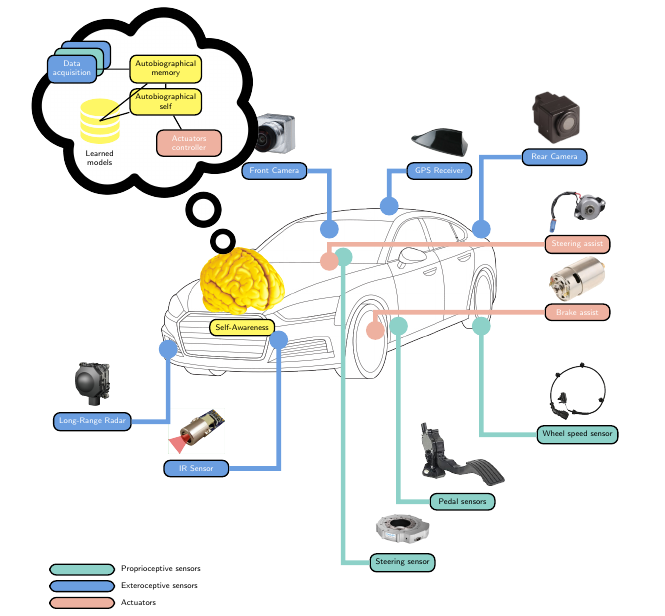
\includegraphics[width=0.7\textwidth]{/media/donkarlo/Elements/projs/research/assets/regazzoni-2020-multi-sensorial-generative-and-descriptive-self-awareness-models-for-autonomous-systems-fig-1.png}
			\caption{\citet{regazzoni-2020-multi-sensorial-generative-and-descriptive-self-awareness-models-for-autonomous-systems}}
			\label{fig:regazzoni-2020-multi-sensorial-generative-and-descriptive-self-awareness-models-for-autonomous-systems-fig-1.jpg}
		\end{figure*}
		
		\paragraph{SA introspection}  The SA representation obtained by jointly and dynamically analyzing the sensory data endows the agent with introspection at different hierarchical levels.
		
		\paragraph{Introspection} associates with the agent’s capability of estimating and
		representing \emph{dynamical causal relationships} from the observed sensory data. Such representation allows the agent to model interactions between itself, as observed through proprioceptive
		sensors; and the environment, as observed through exteroceptive sensors.
		
		\paragraph{importance of embodying SA capabilities}The extent of the embodied SA capabilities influences the agent's performance when solving tasks and are assumed as reasons for the significant capability differences of the various biological species. 
		
		\paragraph{Minimum requirements to consider an agent self-aware}The following capabilities as the minimum requirements in to consider an agent self-aware: 
		\begin{itemize}
			\item initialization
			\item inference
			\item anomaly detection
			\item model creation
			\item interface with control
		\end{itemize}
		\citet{regazzoni-2020-multi-sensorial-generative-and-descriptive-self-awareness-models-for-autonomous-systems} Table I describes the proposed SA capabilities and provides a relationship between each of them and biological agents, demonstrating how humans address these capabilities.
		\begin{figure*}
			\centering
			\includegraphics[width=0.7\textwidth]{/media/donkarlo/Elements/projs/research/assets/regazzoni-2020-multi-sensorial-generative-and-descriptive-self-awareness-models-for-autonomous-systems-table-i.png}
			\caption{Table I}
			\label{fig:regazzoni-2020-multi-sensorial-generative-and-descriptive-self-awareness-models-for-autonomous-systems-table-i.jpg}
		\end{figure*}
	\section{bio-inspired self-awareness theories}
		\subsection{Damasio’s model}
			\paragraph{autobiographical memories (AMs)} Neuroscientists such as Damasio \citet{regazzoni-2020-multi-sensorial-generative-and-descriptive-self-awareness-models-for-autonomous-systems}[28] have provided evidence that neural patterns in the oldest parts of the human brain are organized to process and combine proprioceptive and exteroceptive sensorial information according to hierarchical neural layouts culminating into so-called \emph{autobiographical memories (AMs)}. 
			\\
			AMs can constitute a sort of database for memorizing models of \textbf{episodes} that the agent has learned from previous experiences \citet{regazzoni-2020-multi-sensorial-generative-and-descriptive-self-awareness-models-for-autonomous-systems}[5]. 
			\\
			Bio-inspired AMs have already been investigated towards implementing self-awareness in
			artificial agents, for example, in \citet{regazzoni-2020-multi-sensorial-generative-and-descriptive-self-awareness-models-for-autonomous-systems}[29]. Based on anatomical observations, Damasio suggests that episodes in AMs are \textbf{represented by a language coding proprioceptive and exteroceptive information according to a temporally ordered causal representation.} Fig. 2 depicts the combination of estimations
			of the agent’s own the external world’s state obtained by an
			early neural layout (named “proto” and “core”, respectively)
			in the form of temporal-causal AM patterns.
			\begin{figure*}
				\centering
				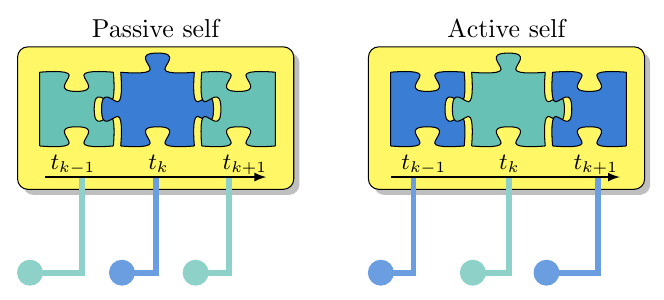
\includegraphics[width=0.7\textwidth]{/media/donkarlo/Elements/projs/research/assets/regazzoni-2020-multi-sensorial-generative-and-descriptive-self-awareness-models-for-autonomous-systems-fig-2.png}
				\caption{regazzoni-2020-multi-sensorial-generative-and-descriptive-self-awareness-models-for-autonomous-systems-fig-2.png}
				\label{fig:regazzoni-2020-multi-sensorial-generative-and-descriptive-self-awareness-models-for-autonomous-systems-fig-2.png}
			\end{figure*}
			\paragraph{} According to Damasio, AM patterns are based on \emph{first-person situational descriptors} that enable human agents to represent experienced episodes on the basis of a \textbf{neural vocabulary} (i.e., information units). These descriptors always represent exteroceptive data as contextualized to information coming from the agent's body, and vice versa. Thus, patters encoding episodic experiences are represented by coupling the agent and its dynamic interaction with the surrounding environment.
			\\
			Elementary information units used in AMs define a temporal
			representation where an agent and the environment reciprocally take on the role of a \emph{context}. Temporal changes of
			the internal representation of the state of one of them (that
			Damasio calls “dispositions”) are observed as occurring in the
			context of the other one assuming a given state (see Fig. 2). Sequences of such patterns are stored in the AM representing
			episodes. Therefore, at least in humans and biological agents,
			SA is based on a \textbf{contextual} representation, which is essential
			for the emergence of the expected SA capabilities as listed in
			\citet{regazzoni-2020-multi-sensorial-generative-and-descriptive-self-awareness-models-for-autonomous-systems} Table I.
			
			\paragraph{Key element in SA knowledge}A dynamic description of agent and environment changes
			based on their reciprocal states is a key element for the
			representation of SA knowledge. This is different from many
			traditional AI systems, where exteroceptive sensory data se-
			quences are often represented at a primary level \emph{without explicit contextual} information. 
		
			\textbf{Traditional AI systems do not consider contextual data}: This is different from many
			traditional AI systems, where exteroceptive sensory data sequences are often represented at a primary level \emph{without explicit contextual information}. As a \textbf{consequence}, high-level
			processing techniques, for example, classifiers based on supervised labeled learning [30], [31], [32], use implicit contextual information to cluster such data into homogeneous groups.
			
			\textbf{A problem}: Despite the impressive classification performance that can be
			achieved when testing data and training experiences belong to
			the same class, the observing artificial agent cannot reliably
			connect such classification results to its internal dynamical
			state when performing similar actions to the ones performed
			during training, simply because its state was not observed and
			memorized together with the observed exteroceptive data. It is therefore not trivial to use such classifiers as building blocks for an artificial agent due to the limited adaptability. 
			
			\paragraph{} Damasio [28] proposed dispositional units, i.e., information units representing contextualized state changes of the
			agent or the environment, for modeling “\textbf{cognitive cycles}”,
			i.e., episodes that can be found as the \emph{basis of human self-awareness}. Moreover, he suggests that dispositional units can
			be hierarchically organized at different levels in the brain, for
			example for describing \emph{temporal-causal} representations in the
			activation and processing results of neuron maps dedicated to
			different goals. Consequentially, an AMs should be hierarchical structured for providing SA models, and thus dispositional
			units’ representations should be defined such that they can be organized in multi-level hierarchies (see Fig. 3).
			\begin{figure*}
				\centering
				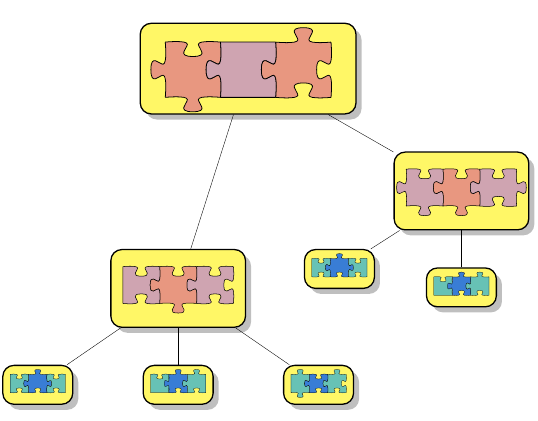
\includegraphics[width=0.7\textwidth]{/media/donkarlo/Elements/projs/research/assets/regazzoni-2020-multi-sensorial-generative-and-descriptive-self-awareness-models-for-autonomous-systems-fig-3}
				\caption{regazzoni-2020-multi-sensorial-generative-and-descriptive-self-awareness-models-for-autonomous-systems-fig-3}
				\label{fig:regazzoni-2020-multi-sensorial-generative-and-descriptive-self-awareness-models-for-autonomous-systems-fig-3.png}
			\end{figure*}
			
			\paragraph{Autobiographical self} Neuroscience observations show that the parts of the human
			brain storing AMs are linked and can exchange neural signals
			with other parts of the brain known to be activated within conscious inference processes [33]. The role of such neural maps
			is to analyze—at different hierarchical levels—proprioceptive
			and exteroceptive sensorial data originating from the current
			agent’s experiences. The process of \emph{recalling} and \emph{comparing
			multi-level AMs}\emph{ with respect to current experiences} is an
		\emph{integral capability} of self-awareness related to inference and
			anomaly detection, which is defined by Damasio as \textbf{autobiographical self} (AS).
			\paragraph{Application of AS}The AS allows an agent to evaluate whether the current experience matches any episode stored in the AM.  Moreover, the AS must provide inference processes to interface with other
			parts of the agent’s brain (e.g., blocks dedicated to agent’s
			resource planning and control of actuators) to maintain a
			dynamic stability condition, i.e., homeostasis \citet{regazzoni-2020-multi-sensorial-generative-and-descriptive-self-awareness-models-for-autonomous-systems}[34]. 
			
			In a SA model, the \underline{inference capability} implies that activated AMs’ dispositional units and currently experienced data elaborated by early neural maps can be managed by the AS inference
			process to perform, for example, predictions on the agent’s
			future states. Based on the temporal-causal organization of
			the available episodes stored in the AM, the AS is able to
			predict future states at multiple abstraction levels by using
			generative models that represent possible alternative realizations of episodes already experienced adapted to currently observed data. As multiple episodes are stored in the AM, the AS inference processes need to identify models that better match the current experience, which requires the dispositional units’ representation in a SA model to inherently provide a discriminative property to assess current data characteristics.
			
			
			\paragraph{in AI} An artificial AS is also required to determine the difference
			between episodes contained in its own AMs and the current
			experiences based on an appropriate metric, which can be interpreted as the basis for the abnormality detection capability
			(see Fig. 4). 
			\begin{figure*}
				\centering
				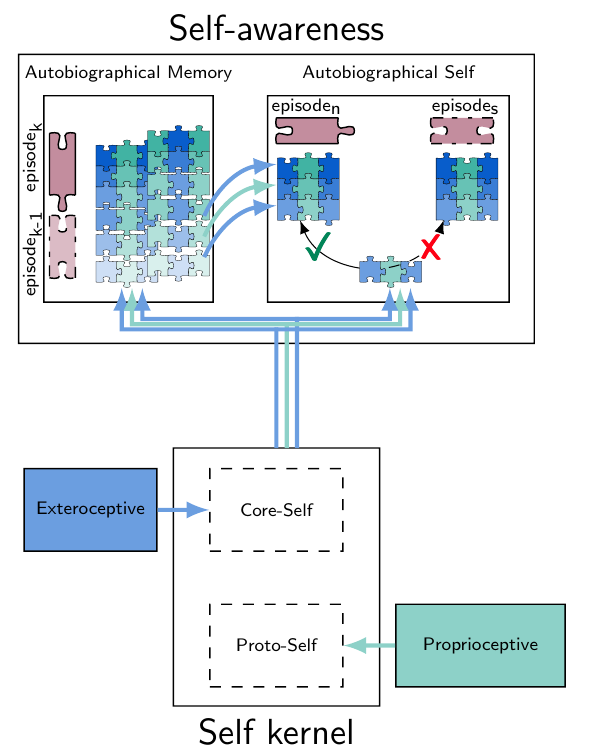
\includegraphics[width=0.7\textwidth]{/media/donkarlo/Elements/projs/research/assets/regazzoni-2020-multi-sensorial-generative-and-descriptive-self-awareness-models-for-autonomous-systems-fig-4.png}
				\caption{Fig. 4: Autobiographical memory (AM) and autobiographical
					self (AS) as core components of a self-aware agent founded
					on Damasio’s model. The core-self and the proto-self process
					exteroceptive and proprioceptive information and store them
					as dispositional units in the AM. The AS is able to perform
					inference and anomaly detection based on the stored episodes.
				}
				\label{fig:regazzoni-2020-multi-sensorial-generative-and-descriptive-self-awareness-models-for-autonomous-systems-fig-4.png}
			\end{figure*}
			
			In order to assess the matching degree between
			predictions derived from the dispositional units of the set of
			potentially applicable episodes and the current observations,
			the SA agent must apply a computable metric invariant to the
			sensor modality. In this case, the agent should be aware that an
			abnormality, i.e., a non-stationary condition never experienced
			before, is currently present. Damasio does not address which
			specific computational neural characteristic included in the
			neural implementation is able to realize such computational
			behavior. He only suggests that such matching and prediction
			inference capabilities can be performed by the AS at different
			abstraction and temporal levels and so enabling an efficient
			selection of the hierarchical and dispositional representation
			of AMs episodes).
			\paragraph{Rise of emotions} It is worth mentioning that for natural agents, Damasio
			suggests that the integrated SA system composed by AM and
			AS can also be used as a possible explanation of higher-level
			human regulatory psychological phenomena such as emotions
			and feelings [35]. Emotions and feelings can be considered
			as emergent results of evaluating current experiences based
			on multi-level hierarchical AMs by means of the AS [25].
			For example, fear can emerge from the capability of detecting
			abnormalities, recognizing that the current experience does not
			match with past AMs, or it matches with AMs that describe
			dangerous episodes. Damasio’s model implicitly implies that
			AS outcomes enable an agent to incrementally update in-
			ternal AM models by coding abnormal experiences into new
			models as well as to define a SA system that derives inferences
			invariant to the involved sensor modalities.
			
			
		\subsection{Haykin’s model}
		
		In comparison with Damasio’s work, Haykin proposes a
		computational framework of neuroscience observations from
		an engineering perspective referred to as \textbf{Cognitive Dynamic
		Systems (CDS)} [36]. The proposed CDS model is based on the
		interactions that a \emph{Cognitive Controller} (CC) part of a CDS has
		to maintain at multiple levels of abstractions with a \emph{Cognitive Perceptor(CP)}. 
		
		The CP processes exteroceptive information
		coming from the environment at different hierarchical levels
		and can be seen as a hierarchical probabilistic filter, generating environment descriptions at different abstraction levels.
		\\
		Beyond providing information to higher levels, such a filter
		generates hierarchical feedback information to the CC, which
		in turn computes commands to actuators that are characterized
		by uncertainty. The CC block of Haykin’s model is described
		as a top-down structure generating outputs towards lower
		levels. \emph{At the bottom layer}, it directly generates outputs for
		the \emph{actuators}.
		\\
		The \emph{Probabilistic Reasoning Machine} (PRM), introduced
		in a joint paper with J. Fuster [37], organizes probabilistic
		information coming from the CP, i.e., percepts and errors
		(prediction and update processes), together with information
		coming from the CC, i.e., planned actions with its related
		uncertainty. Such an organization is performed over time.
		As can be seen in Fig. 5, Haykin’s model does \emph{not directly
		employ proprioceptive} sensory data but uses internal strategies
		to generate commands towards actuators.
		\begin{figure*}
			\centering
			\includegraphics[width=0.7\textwidth]{/media/donkarlo/Elements/projs/research/assets/regazzoni-2020-multi-sensorial-generative-and-descriptive-self-awareness-models-for-autonomous-systems-fig-5.png}
			\caption{Fig. 5: Hierarchically structured probabilistic reasoning machine (PRM) adopted from [37]. The cognitive perceptor (CP) processes exteroceptive information (“percepts”) at different hierarchical levels, and the cognitive controller (CC) generates outputs towards the actuators in a top-down structure. The PRM organizes probabilistic information from perception and control by data structures capturing causal-temporal interactions that are similar to “dispositional units”.
			}
			\label{fig:regazzoni-2020-multi-sensorial-generative-and-descriptive-self-awareness-models-for-autonomous-systems-fig-5.png}
		\end{figure*}
		The \textbf{main goal} of the PRM is to maintain a meta-level representation of the \emph{perception-action} cycle based on switching and adapting the behavior of CP and CC.
		
		\paragraph{The relation between Haykin and Damasio}As the control strategies embedded in the CP are hypothesized to maintain homeostasis, i.e., a dynamic equilibrium between the agent’s state and the changes in the environment, the PRM is contributing
		to the continuous regulation of agents’ processes by providing
		switching suggestions to CP and CC. Those suggestions are
		implicitly based on the knowledge that an agent must have
		been learned from experiences, and it is represented within
		the PRM. \textbf{In this sense, the PRM block is strictly related to
		Damasio’s SA model}, as it has to process representations of
		actions and percepts organized in a \textbf{temporal-causal} order, and
		the \emph{PRM block can be related to AM and AS as SA} model
		capabilities.
		\paragraph{} The PRM elementary representation requires organizing
		perception and actions into data structures capturing causal
		and temporal interactions between the agent’s actions and
		percepts originated from the environment. Dispositional information units, as described by Damasio, also represent such
		interactions but are different because the state of the agent
		is directly observed by itself. This can be considered either
		as feedback for the SA agent to evaluate the outcome of
		commands it has sent to actuators and lower-level blocks or
		as a multi-sensor source of proprioceptive signals representing
		the agent state to itself. This concept is exploited in \cite{regazzoni-2020-multi-sensorial-generative-and-descriptive-self-awareness-models-for-autonomous-systems} SA
		model (depicted in Fig. 10). If this second view is taken,
		a modified PRM can be considered as a structure where
		appropriately modified dispositional units are processed based
		on hierarchical filters that work on proprioceptive feedback
		and in a bottom-up way also in the CC.
		\paragraph{} In Haykin’s approach, the \emph{focus is on control} instead of SA.
		Therefore, the PRM is designed to make a CDS capable of
		using interactive behavioral rules to switch among different
		perceptions and action modalities adaptively. Such inferences
		can drive actions that the agent’s sensors and actuators should
		accomplish anticipatorily by activating available models in
		the PRM memory when it performs a given experience. This
		allows the CDS of an attention capability towards preferred
		control or sensing actions in a given homeostatic cycle. In the
		case of the SA model discussed here, the agent has no direct
		knowledge of the control strategy actions that are generated
		by its own decision-making subsystem, but it can observe and
		fuse their outcomes through parallel proprioceptive feedback
		from sensors coupled with exteroceptive environmental observations. Haykin’s model, however, suggests how a SA model
		can provide useful data to adapt decision making processes
		behaviors at homogeneous hierarchical levels to the PRM.
		For example, SA can share with decision-making estimates
		of present and predicted contextualized states as well as
		errors and deviations of models describing previous agent
		experiences.
		\paragraph{}Furthermore, Haykin’s model facilitates identifying temporal variations of uncertainty associated with actions and
		percepts, which is a key aspect for addressing a proper
		computational framework for the CDS design, i.e., a PRM
		in \cite{regazzoni-2020-multi-sensorial-generative-and-descriptive-self-awareness-models-for-autonomous-systems} SA model. Moreover, the organization of a PRM at
		multiple abstraction levels is coherent with the hierarchical
		characteristics of Damasio’s dispositional units. In this case,
		actions and percepts as temporal aggregations (equivalent to
		dispositional units) at different hierarchical levels can describe
		the joint state of lower-level parts of the agent body down
		to the directly observed proprioceptive and exteroreceptive
		characteristics of the agent and the environment. Although
		Haykin’s approach does not provide a specific probabilistic model for uncertainties and dependencies, it proposes a
		Bayesian framework to model uncertainty and causality and
		make inferences computationally, e.g., parametric conditional
		probability models.
		
		\paragraph{}Although the goal of Haykin is not to specify a univocal
		PRM model but to provide a generic framework for CDSs, his
		model is essential for addressing the main techniques for SA in
		artificial agents. His work then suggests that SA models origi-
		nating from a computational domain should be associated with
		an appropriate calculus of uncertainty propagation. In [38], a
		CDS inspired by such a probabilistic approach uses a simple
		PRM unit that allows a vision system on a mobile platform to
		make inferences about future states. Moreover, Haykin’s work
		does not directly provide a unitary view of the techniques
		that could be used to store a coherent multi-level generative
		and discriminative PRM’s knowledge. Nonetheless, \cite{regazzoni-2020-multi-sensorial-generative-and-descriptive-self-awareness-models-for-autonomous-systems} work
		integrates Haykin’s viewpoint on uncertainty and makes a
		relation between the perception-control blocks and Damasio’s
		theory, which includes AM and AS and dispositional units.
		\cite{regazzoni-2020-multi-sensorial-generative-and-descriptive-self-awareness-models-for-autonomous-systems}Fig. 10 displays a revisited block scheme of Haykin’s model.
		
		\subsection{Friston’s model}
		Another relevant cognitive framework for SA that aims at
		establishing links between neuroscientific observations and
		computational models is the one proposed by Friston [39],
		[27]. Here, Bayesian dynamical systems are the computational
		tool that facilitates an uncertain and hierarchical self-
		coherent representation to describe and generate simulations
		of inferences performed by the human brain utilizing neuron
		firings. Friston’s approach is innovative in the context of
		developing self-aware models for artificial agents due to the
		following characteristics: i) It formally relates a statistical me-
		chanics’ optimization framework, that can be summarized as
		free energy and variational based reasoning, with Bayesian
		inference. It founds a theoretical domain for describing SA
		knowledge and models (in the AM) as well as inference (in
		the AS). ii) It proposes the concept of generalized states (GS)
		to develop a class of computational and hierarchical Bayesian
		filters that we use to embed representation and inference over
		dispositional temporal knowledge.
		\paragraph{} The good regulator theorem [35] states that “every good
		regulator of a system must be a model of that system”. In this
		sense, SA models can be considered as joint discriminative
		and generative models that contribute to the regulation of an artificial agent representing an adaptive code of the system
		itself and its incremental experiences at the same time. The
		free energy principle represents an optimization criterion that
		can be related with a variational computational framework to
		both define and discover optimal SA models from a given
		set of dynamic experiences, i.e., available data sequences
		originating from exteroceptive and proprioceptive sensors.
		\paragraph{} In [27], Friston suggests that establishing an equivalence
		between a probabilistic and a mechanical statistics’ representation of the dynamic equilibrium in the sensed internal
		state and the contextual environment allows one to explain
		the observed neuron firing in the human brain through the free
		energy concept. He further shows that Bayesian inference is an
		equivalent way to do so. As SA in humans is based on brain
		inference processes, probabilistic dynamic representation and
		inference models are good candidates to form the \textbf{language}
		for expressing a SA model in an artificial agent as well. Such
		models must be capable of including temporally ordered descriptions of contextual dependencies between proprioceptive
		and exteroceptive variables.
		\paragraph{} The variational computational representation and inference
		techniques he proposes clarify how different models can
		describe statistically different sensorial experiences that can
		be seen as trajectories in generalized spaces. The models
		can also provide explicit measurements to evaluate or to
		discriminate best-fitting models of new observed sequences.
		At the same time, the same models, that can include multiple conditionally connected random variables at different
		hierarchical and temporal levels, are capable of predicting
		multi-level, temporal data series characterized by the same
		statistical properties of the training experiences from which
		they can be learned (thanks to their generative nature). Such
		a model, if used within the SA model of an artificial agent,
		together with appropriate learning techniques, can facilitate
		incremental model creation. An AS can so actively memorize
		incrementally generative and discriminative new models in the
		AM by processing sensorial experiences. Such models have to
		capture different causality interactions between the agent and
		the environment and serve as the basis for \emph{symbolic} descriptors
		in an artificial SA agent.
		\paragraph{} The SA capability of abnormality detection can also be
		explained with Friston’s model, i.e., the free energy that
		models generate when the AS compares them to a new
		experience. A metric can be defined to evaluate the amount
		of abnormality which is related to a particular component
		of free energy, describing the orthogonal perturbations to the
		dynamic equilibrium condition described by the model. Such
		a metric enables the AS to rank the abnormalities measured
		from a set of AM models, so relating the discriminative
		SA property of the model to the abnormality detection and
		inference capabilities.
		\paragraph{}Contribution ii) to the SA model definition is a specific class
		of Bayesian filters, namely GS filters. Friston et al. [40] explain
		that thanks to such filters, active and variational Bayesian
		inference techniques can be obtained with better performances.
		GSs describe a class of trajectories in terms of generalized
		coordinates of motion. The resulting model can be shown to
		better describe the dynamical nature of the pattern in terms
		of temporal and causal explainability of dependencies among
		states as well as computational benefits. In a SA model,
		hierarchical Bayesian models derived from GS filters can
		provide the description language for the AM, depicted as
		individual “pages” in Fig. 6. \citet{regazzoni-2020-multi-sensorial-generative-and-descriptive-self-awareness-models-for-autonomous-systems} shows how these models
		can be learned by observing proprioceptive and exteroceptive
		data series both independently and in a coupled way that is
		oriented to represent their dispositional nature. Such filters can
		be used both as generative and discriminative models, and they
		can be good candidates to be related to the “good regulator”
		code [35], as they can represent the rules that describe the
		agent, as well as such rules, can be used by the agent to predict
		the dynamic contextualized behavior where it is acting.
		\begin{figure*}
			\centering
			\includegraphics[width=0.7\textwidth]{/media/donkarlo/Elements/projs/research/assets/regazzoni-2020-multi-sensorial-generative-and-descriptive-self-awareness-models-for-autonomous-systems-fig-6.png}
			\caption{\citet{regazzoni-2020-multi-sensorial-generative-and-descriptive-self-awareness-models-for-autonomous-systems} Fig. 6}
			\label{fig:regazzoni-2020-multi-sensorial-generative-and-descriptive-self-awareness-models-for-autonomous-systems-fig-6.png}
		\end{figure*}
		\paragraph{} Coupled proprioceptive and exteroceptive signals of GS
		filters can efficiently represent Damasio’s dispositional units
		in a SA model. For example, a Switching Dynamic Bayesian
		Network (DBN) [41], [42] uses multi-level discrete and con-
		tinuous generalized states as variables that will be further
		discussed in the following sections.
		\paragraph{} Dynamic Expectation Maximization (DEM) filters [40] are
		hierarchical parametric GS filters that are here used to
		derive coupled GS-DBNs. These filters have been shown to
		jointly perform parameter, hyperparameters, and GS estimations within a continuous variable Bayesian network that is
		by itself a fully continuous DBN. However, discrete variables
		are needed in a SA model too. Such variables are used to
		represent different models (i.e., different pages in the AM
		structure) and to provide finer level discriminative descriptions
		of learned models to determine a different class of probabilistic
		dependencies within an episode, useful both for generative
		and discriminative purposes. Coupled GS-DBNs are, therefore,
		better-suited filters than DEM, in particular when all model
		properties are necessary to reach the SA capabilities (see
		Fig. 7).
		\begin{figure*}
			\centering
			\includegraphics[width=0.7\textwidth]{/media/donkarlo/Elements/projs/research/assets/regazzoni-2020-multi-sensorial-generative-and-descriptive-self-awareness-models-for-autonomous-systems-fig-7.png}
			\caption{\cite{regazzoni-2020-multi-sensorial-generative-and-descriptive-self-awareness-models-for-autonomous-systems}Fig. 7}
			\label{fig:regazzoni-2020-multi-sensorial-generative-and-descriptive-self-awareness-models-for-autonomous-systems-fig-7.png}
		\end{figure*}
	
	\section{ SIGNAL REPRESENTATION AND MODEL LEARNING}
		\subsection{Bio-inspired SA Model}
		The main difference between Haykin’s and Damasio’s models is that the objective of the latter lies in the bottom-up
		explanation of neuroscientific observations, while the first one
		focuses on the definition of control within a CDS. Similar
		to Haykin’s model, Friston’s approach is based on a Bayesian
		and computationally efficient approach for SA representations.
		Friston’s approach is more focused on a bottom-up joint analysis of proprioceptive and exteroceptive signals, while Haykin’s
		model aims at providing a framework for defining computational aspects of perception-action cycle decision making
		outcomes towards actuators in a CDS. A computational SA
		model for an artificial agent can be obtained by merging
		different aspects of the three frameworks. Such SA model
		should include SA properties as discussed in Section I and
		enlisted in \cite{regazzoni-2020-multi-sensorial-generative-and-descriptive-self-awareness-models-for-autonomous-systems}Table II.
		\begin{figure*}
			\centering
			\includegraphics[width=0.7\textwidth]{/media/donkarlo/Elements/projs/research/assets/regazzoni-2020-multi-sensorial-generative-and-descriptive-self-awareness-models-for-autonomous-systems-table-ii.png}
			\caption{\cite{regazzoni-2020-multi-sensorial-generative-and-descriptive-self-awareness-models-for-autonomous-systems} Table II}
			\label{fig:regazzoni-2020-multi-sensorial-generative-and-descriptive-self-awareness-models-for-autonomous-systems-table-ii.png}
		\end{figure*}
		\paragraph{How to build new models from big errors}
		\citet{regazzoni-2020-multi-sensorial-generative-and-descriptive-self-awareness-models-for-autonomous-systems} Fig. 6 and Fig. \citet{regazzoni-2020-multi-sensorial-generative-and-descriptive-self-awareness-models-for-autonomous-systems} 8 depict how the AM can be represented as
		a book containing \textbf{multiple pages}. Each page corresponds to
		a probabilistic model learned based on observed sequences of
		dispositional units during different experiences. Such a model
		should be both generative and discriminative. 
		\begin{figure*}
			\centering
			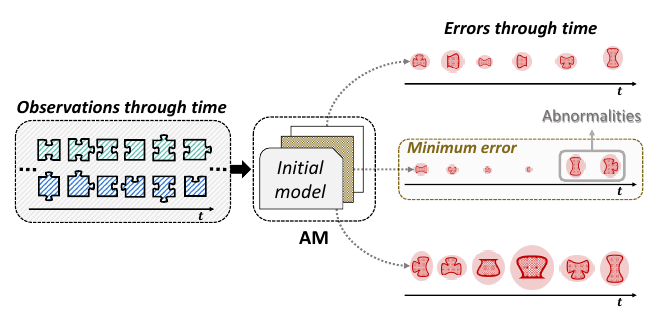
\includegraphics[width=0.7\textwidth]{/media/donkarlo/Elements/projs/research/assets/regazzoni-2020-multi-sensorial-generative-and-descriptive-self-awareness-models-for-autonomous-systems-fig-8.png}
			\caption{\cite{regazzoni-2020-multi-sensorial-generative-and-descriptive-self-awareness-models-for-autonomous-systems} Fig 8 Models in the agent’s memory produce error mea-
				surements as observations arrive. The fittest model is iden-
				tified/discriminated and abnormalities (high errors w.r.t a
				threshold) are extracted from it. Such high errors are then
				used to create new models incrementally as shown in Fig. 6.
			}
			\label{fig:regazzoni-2020-multi-sensorial-generative-and-descriptive-self-awareness-models-for-autonomous-systems-fig-8.png}
		\end{figure*}	
		\paragraph{Basis for initialization} \citet{regazzoni-2020-multi-sensorial-generative-and-descriptive-self-awareness-models-for-autonomous-systems}Fig. 6 shows that
		an initial reference model serves as a \textbf{basis for initialization}.
		This initial model should represent quite general behavioral
		rules obtained in correspondence to a reference experience. For
		example, as \citet{regazzoni-2020-multi-sensorial-generative-and-descriptive-self-awareness-models-for-autonomous-systems} will show, it can contain knowledge useful to
		predict the agent’s state, even if the environment does not interact with it, and therefore exteroceptive signals do not provide
		significant contextual temporal and causal information. In that
		case, the expected agent’s state changes are null, except for
		random perturbations, and state and its derivatives estimated
		from proprioceptive signals can be stationary.
		\paragraph{}The initial model and all generated models in the AM
		must be generative, i.e., they should be capable, under the
		effect of a latent null variable, to generate a sequence of
		predictions in the form of expected probabilistic properties
		of the dispositional unit that could be observed as evidence.
		This has to happen as part of the inference process in the AS
		module. The AS module must be capable of comparing the
		current set of dispositional units from the current experience
		with the predictions of the \textbf{currently \emph{activated} AM page}. This
		comparison has to produce both an evaluation of the \textbf{mismatch
		degree} between predicted and observed dispositional units but
		also to describe such errors and memorizing them for further
		steps. When mismatches are relevant, i.e., abnormalities with
		respect to the initial model are too high, the sequences of
		dispositional units and related errors (generalized errors) are
		processed for describing the \textbf{new experience}. The model creation phase organizes such data series that can be considered
		as sparse acquisitions of generalized errors with respect to
		selected AM available models, e.g., by using unsupervised
		machine learning tools into new models. The results of the
		analysis of the sparse generalized errors are described again
		in terms of behavioral rules expressed using generative models
		with the same language of the initial models. \textbf{Such new models
		can be seen as new pages to be added to the AM book.}
		\textbf{Memorization} includes the capability to organize the learned
		models within the AM model as incremental pages in a book.
		\citet{regazzoni-2020-multi-sensorial-generative-and-descriptive-self-awareness-models-for-autonomous-systems} Section II-B describes how this can be obtained starting from
		free energy and generalizes state concepts in a way inspired
		to Friston’s approach.
		\paragraph{} \citet{regazzoni-2020-multi-sensorial-generative-and-descriptive-self-awareness-models-for-autonomous-systems}Fig. 8 highlights the inference capability of the AS when
		the AM is composed of multiple pages, i.e., to \textbf{discriminatively
		select a page that better fits to the current experience}. Again,
		this can be obtained by comparing the generalized errors obtained by processing in multiple parallel models and evaluating
		when the minimum detected error is sufficiently small. The
		page which produced such a set of generalized error also
		contains the causal and temporal knowledge to predict the
		dynamic evolution of the contextual state of the agent and
		the environment, so providing to the agent a symbolic and
		continuous SA description of what is happening compared
		to past experiences. The minimum abnormality criterion to
		discriminate the most fitting model can be considered as the
		selection of the model characterized by the lowest generalized
		error, evaluated by using an appropriate metric. Therefore, the
		SA discriminative capability results by comparing the current
		experience to the generated predictions of a set of models of
		experiences available at a given moment in an agent. \citet{regazzoni-2020-multi-sensorial-generative-and-descriptive-self-awareness-models-for-autonomous-systems}Fig. 8
		shows how the inference process in the AS can also generate
		useful information for decision making. In particular, the set of predictions and related errors derived from comparing
		activated models with the current dispositional units can be
		used by a decision making block to plan resources usage as
		well as to decide among alternative actuator signals to perform
		planned actions.
		
		\paragraph{} \citet{regazzoni-2020-multi-sensorial-generative-and-descriptive-self-awareness-models-for-autonomous-systems}Fig. 9 shows that, in contrast to Haykin’s theory, the SA
		model does not explain the perception-action cycle, so it
		does not include a hierarchical control block. Instead, pro-
		prioceptive signals provided by observing agent actuators are
		processed in parallel in a bottom-up way with exteroceptive
		signals processed in the block defined as Perception in \citet{regazzoni-2020-multi-sensorial-generative-and-descriptive-self-awareness-models-for-autonomous-systems}[43]. As
		can be seen in \citet{regazzoni-2020-multi-sensorial-generative-and-descriptive-self-awareness-models-for-autonomous-systems}Fig. 10, the PRM is replaced by the SA model
		as it aims to organize extero and proprio percepts, with the
		latter being considered as the feedback generated by actuators
		controls by the agent itself.
		\begin{figure*}
			\centering
			\includegraphics[width=0.7\textwidth]{/media/donkarlo/Elements/projs/research/assets/regazzoni-2020-multi-sensorial-generative-and-descriptive-self-awareness-models-for-autonomous-systems-fig-9.png}
			\caption{\cite{regazzoni-2020-multi-sensorial-generative-and-descriptive-self-awareness-models-for-autonomous-systems} Fig 9 Relationships between exteroceptive states (bottom)
				and generalized states (top). Two consecutive states are ab-
				stracted into a generalized state that has information about i)
				the current state (depicted by the shape of the puzzle piece)
				and ii) its derivative (depicted by the arrows pointing at the
				expected state’s change in the succeeding time instant). Note
				that the same logic can be applied to proprioceptive data (green
				puzzle pieces).
			}
			\label{fig:regazzoni-2020-multi-sensorial-generative-and-descriptive-self-awareness-models-for-autonomous-systems-fig-9.png}
		\end{figure*}
		\paragraph{}For the proposed model to be effective, it must fulfill the
		properties listed in Table II. In particular, \citet{regazzoni-2020-multi-sensorial-generative-and-descriptive-self-awareness-models-for-autonomous-systems} note that the
		content of AM pages represents models organized into random
		variables that should come from observations of dispositional
		units (i.e., interactive variables embedding causal and temporal
		aspects). They are random variables at multiple hierarchical
		levels. Moreover, the SA process has to be autopoietic in
		the sense that it should be able to learn new pages of the
		AM book from computed generalized errors by generating
		predictions from pages already available in the AM book. As a
		function of generalized errors over the generalized state-space
		describes the differences between the current experience and
		the existing AM page, this means that a new page generated
		during model creation should provide a generalized null error,
		i.e., that learning process should be capable of representing a
		function of generalized error over the generalized state space
		as a book page model.
		
		
	
	
	
	
	
	\bibliography{/media/donkarlo/Elements/projs/research/refs}
\end{document}